\documentclass{standalone}
\usepackage{tkz-fct}
\usepackage{tkz-euclide}
\usepackage{color}
\renewcommand*\familydefault{\sfdefault}
\usepackage{sansmath}
\usepackage{amsmath}
\sansmath
\definecolor{gray75}{gray}{0.75}
\begin{document}
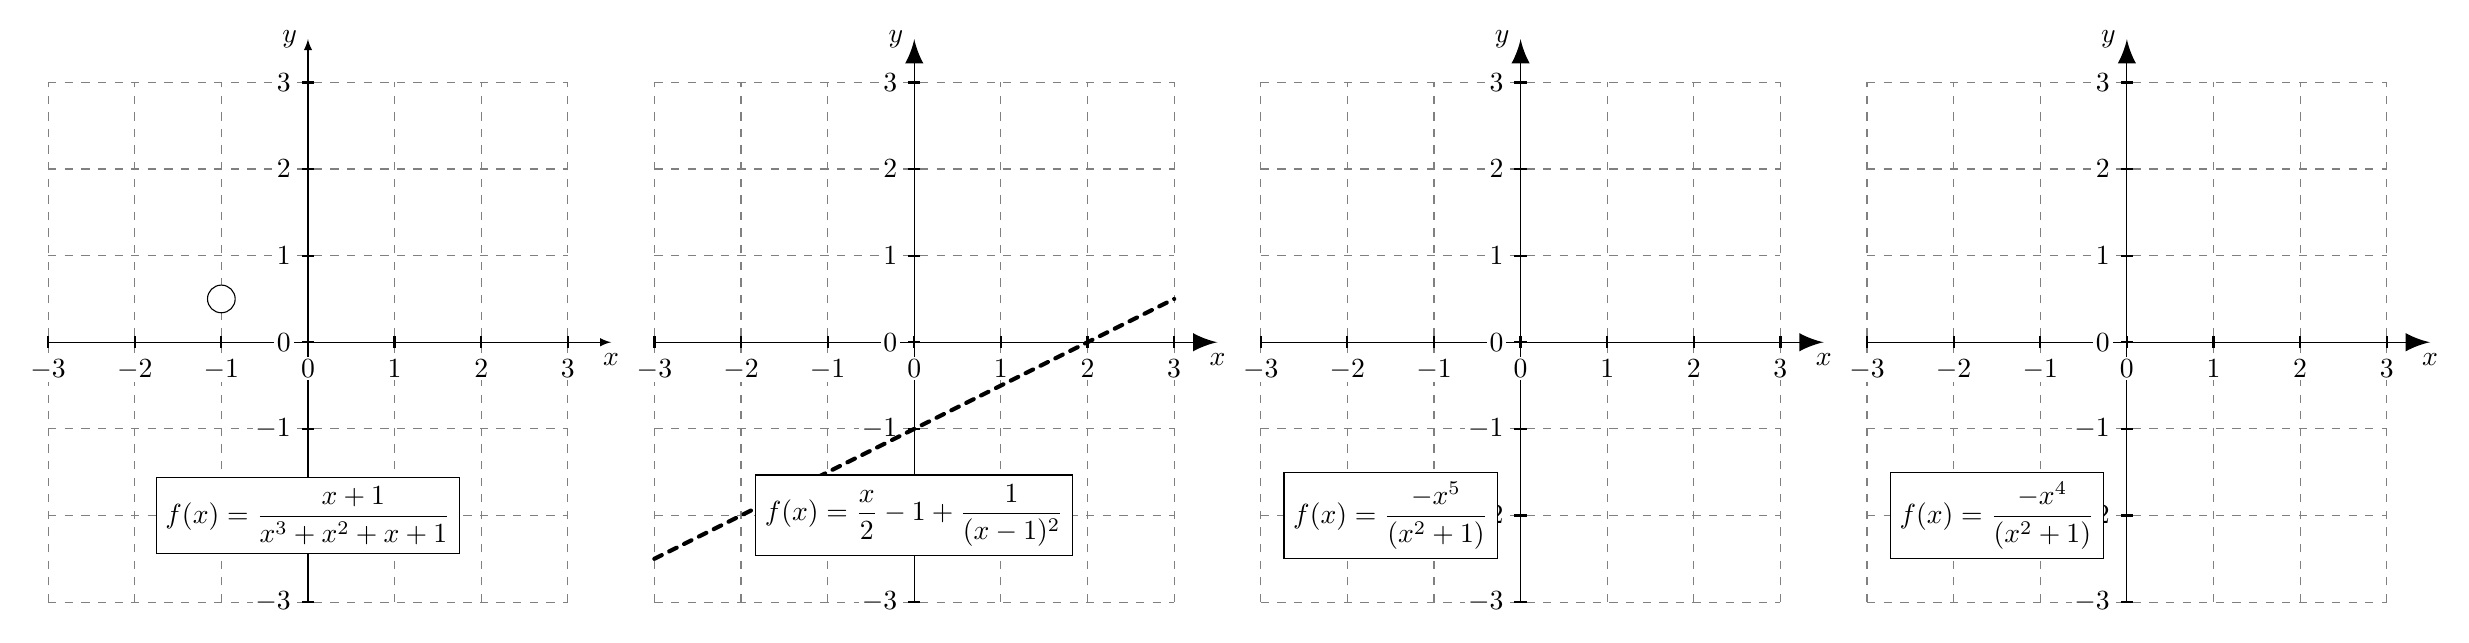
\begin{tikzpicture}[scale=1.1]
  \tkzInit[xmin=-3, xmax=3,ymin=-3,ymax=3]
  \begin{scope}[dashed]
    \tkzGrid
  \end{scope}
  \tkzDrawX[label={$x$}]
  \tkzDrawY[label={$y$}]
  \tkzLabelX
  \tkzLabelY
  \tkzFct[line width=2pt, domain=-3:3]{(x+1)/(x**3+x**2+x+1)}
  \tkzDrawPoint[size=10,color=black,fill=white](-1.0,0.5)
  \tkzText[draw,
  fill=white](0,-2){$f(x)=\dfrac{x+1}{x^{3}+x^{2}+x+1}$}
  \begin{scope}[xshift=7cm]
\tkzInit[xmin=-3, xmax=3,ymin=-3,ymax=3]
  \begin{scope}[dashed]
    \tkzGrid
  \end{scope}
  \tkzDrawX[label={$x$}]
  \tkzDrawY[label={$y$}]
  \tkzLabelX
  \tkzLabelY
  \tkzFct[line width=2pt, domain=-3:0.9]{0.5*x-1+1/(x-1)**2}
  \tkzFct[line width=2pt, domain=1.1:3]{0.5*x-1+1/(x-1)**2}
  \tkzDefPoint(-3.0,-2.5){A}
  \tkzDefPoint(3.0,0.5){B}
  \tkzDrawSegment[style=dashed,line width = 1.5pt](A,B)
  \tkzText[draw, fill=white](0,-2){$f(x)=\dfrac{x}{2}-1+\dfrac{1}{(x-1)^{2}}$}
\end{scope}
\begin{scope}[xshift=14cm]
\tkzInit[xmin=-3, xmax=3,ymin=-3,ymax=3]
  \begin{scope}[dashed]
    \tkzGrid
  \end{scope}
  \tkzDrawX[label={$x$}]
  \tkzDrawY[label={$y$}]
  \tkzLabelX
  \tkzLabelY
  \tkzFct[line width=2pt, domain=-3:1]{-x**5/(x**2+1)}
  \tkzFct[line width=2pt, domain=1:3]{-x**5/(x**2+1)}
  \tkzText[draw, fill=white](-1.5,-2){$f(x)=\dfrac{-x^{5}}{(x^{2}+1)}$}
\end{scope}
\begin{scope}[xshift=21cm]
\tkzInit[xmin=-3, xmax=3,ymin=-3,ymax=3]
  \begin{scope}[dashed]
    \tkzGrid
  \end{scope}
  \tkzDrawX[label={$x$}]
  \tkzDrawY[label={$y$}]
  \tkzLabelX
  \tkzLabelY
  \tkzFct[line width=2pt, domain=-3:1]{-x**4/(x**2+1)}
  \tkzFct[line width=2pt, domain=1:3]{-x**4/(x**2+1)}
  \tkzText[draw, fill=white](-1.5,-2){$f(x)=\dfrac{-x^{4}}{(x^{2}+1)}$}
\end{scope}
\end{tikzpicture}
\end{document}
